\documentclass[12pt]{article}
% Full article preamble (duplicated, no common file)
\usepackage{fontspec}
\usepackage[a4paper,margin=2.5cm,includefoot]{geometry}
\usepackage{polyglossia}
\usepackage{amsmath}
\usepackage{amssymb}
\usepackage{xcolor}
\usepackage{fancyhdr}
\usepackage{graphicx}
\usepackage{listings}
\usepackage[most]{tcolorbox}
\usepackage{pifont}
\usepackage{enumitem}
\usepackage{titlesec}
\usepackage[bottom]{footmisc}
\usepackage{titling}
\usepackage{minted}
\usepackage{etoolbox}
\usepackage{array}
\usepackage{extsizes}

\newfontfamily\emoji{Segoe UI Emoji}

\pagestyle{fancy}

\setmainlanguage[numerals=western]{arabic}
\setotherlanguage{english}
\newfontfamily\arabicfont[Script=Arabic]{Amiri}
\newfontfamily\arabicfonttt[Script=Arabic]{Courier New}

\lstset{
  language=[Sharp]C,
  numbers=left,
  stepnumber=1,
  numbersep=8pt,
  frame=single,
  basicstyle=\ttfamily\small,
  keywordstyle=\color{blue},
  stringstyle=\color{red},
  commentstyle=\color{green!50!black}
}

\newif\ifdetailed
\ifdefined\setdetailed
  \setdetailed
\fi

\newif\ifwithsols
\ifdefined\setwithsols
  \setwithsols
\fi

% unified tcolorboxes for articles
\tcbset{colback=white, colframe=black, fonttitle=\bfseries, boxrule=0.8pt}
\newtcolorbox{boxDef}[1][]{colback=blue!5!white,colframe=blue!75!black,
  title={{\emoji📘} تعريف\ifx\\#1\\\else ~#1\fi :}}
\newtcolorbox{boxExercise}[1][]{colback=cyan!5!white,colframe=cyan!70!black,
  title={{\emoji🧩} تمرين\ifx\\#1\\\else ~#1\fi :}}
\newtcolorbox{boxExample}[1][]{colback=yellow!5!white,colframe=orange!90!black,
  title={{\emoji📝} مثال\ifx\\#1\\\else ~#1\fi :}}
\newtcolorbox{boxNote}[1][]{colback=gray!10!white,colframe=black,
  title={{\emoji✨} ملاحظة\ifx\\#1\\\else ~#1\fi :}}
\newtcolorbox{boxAttention}[1][]{colback=magenta!10!white,colframe=magenta!80!black,
  title={{\emoji🔔} تنبيه\ifx\\#1\\\else ~#1\fi :}}
\newtcolorbox{boxWarning}[1][]{colback=red!5!white,colframe=red!75!black,
  title={{\emoji⚡} ملاحظة هامة\ifx\\#1\\\else ~#1\fi :}}
\newtcolorbox{boxSolution}[1][]{colback=green!5!white,colframe=green!60!black,
  title={{\emoji✅} حل\ifx\\#1\\\else ~#1\fi :}}
\newtcolorbox{boxSymbol}[1][]{colback=purple!5!white,colframe=purple!70!black,
  title={{\emoji🔣} رمز\ifx\\#1\\\else ~#1\fi :}}

\tcbset{simplecode/.style={ colback=gray!5, colframe=black!50, boxrule=0.4pt, arc=2pt, left=4pt,right=4pt,top=4pt,bottom=4pt}}
\newenvironment{boxCode}{\begin{tcolorbox}[simplecode]}{\end{tcolorbox}}

\newcolumntype{C}[1]{>{\centering\arraybackslash}p{#1}}

% redefine spaces after titles
\makeatletter
\renewcommand{\@maketitle}{%
  \begin{center}
    {\huge \bfseries \@title \par}%
    \vskip 0.2em % space between title and author
    {\large \@author \par}%
    % \vskip 0.2em % space between author and date
    % {\normalsize \@date \par}%
  \end{center}
}
\makeatother

\fancyhf{} % clear default
\fancypagestyle{plain}{
  \fancyhf{}
  \fancyhead[L]{مدرسة التسامح الشاملة}
  % \fancyhead[L]{
\includegraphics[height=1cm]{../../../images/logoTasamoh.png}}
  \fancyhead[R]{الأستاذ محمود اغبارية}
  \fancyfoot[C]{\thepage}
}

\fancyhead[L]{مدرسة التسامح الشاملة}
\fancyhead[R]{الأستاذ محمود اغبارية}
\fancyfoot[C]{\thepage}
% \date{\today}

\setcounter{tocdepth}{3} % only section subsection and subsubsection in TOC


% ----------------------


% \begin{document}

% \maketitle

% % \clearpage  % start TOC on a new page
% % \renewcommand{\contentsname}{جدول المحتويات}
% % \tableofcontents
% % \clearpage

% \part*{part 1} % the * prevents numbering
% \section*{مقدمة}
% \subsection*{مثال رياضي}
% \subsubsection*{مثال فرعي}
% \paragraph*{ paragraph 1}
% \subparagraph*{sub paragraph 1}

% \ifdetailed
% \begin{english}
% \begin{minted}{csharp}
% // C# Example
% \end{minted}
% \end{english}
% \fi

% OLD WAY
% \ifdetailed
% \begin{english}
% \begin{lstlisting}
% // C# Example
% \end{lstlisting}
% \end{english}
% \fi

% % 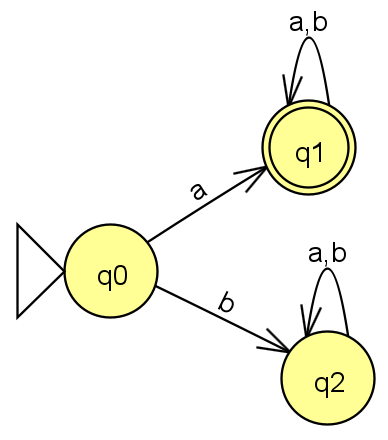
\includegraphics[width=0.2\textwidth]{../../../images/DFAs/ex1_q1.png}



% \vspace{3cm}
% \begin{flushleft}
% أرجو لكم وقتًا ممتعًا.

% الأستاذ محمود اغبارية.
% \end{flushleft}


% \end{document}


\title{ورقة تمرن 5 للصف العاشر 10 - عمليات خارجية}

\begin{document}

\maketitle
\thispagestyle{fancy}

\ifwithsols
\begin{enumerate}[itemsep=3em]
\else
\begin{enumerate}
\fi



\begin{boxAttention}
عندما يٌطلب "عملية خارجية \textbf{تستقبل}" يجب ان يكون المستخدم يدخل قيمة للمتغير. أي عليك استعمال \texttt{Console.ReadLine()}. \\


أما عندما يُطلب منك "عملية خارجية \textbf{تتلقى}" فهذا يعني أنّها تتلقى المطلوب كبارمترات.
\end{boxAttention}

\item اكتب عملية خارجية \textbf{تستقبل} اسم المستخدم \textbf{وتطبع} اسمه.
\ifwithsols
\begin{boxSolution}
\begin{english}
\begin{minted}{csharp}
public static void PrintNameReceive()
{
    string name = Console.ReadLine();
    Console.WriteLine(name);
}
public static void Main()
{
    PrintNameReceive();
}
\end{minted}
\end{english}
\end{boxSolution}
\clearpage
\fi


\item اكتب عملية خارجية \textbf{تستقبل} اسم المستخدم \textbf{وتعيد} اسمه.
\ifwithsols
\begin{boxSolution}
\begin{english}
\begin{minted}{csharp}
public static string ReadNameReturn()
{
    string name = Console.ReadLine();
    return name;
}
public static void Main()
{
    string name = ReadNameReturn();
    Console.WriteLine(name);
}
\end{minted}
\end{english}
\end{boxSolution}
\fi


\item اكتب عملية خارجية \textbf{تتلقى} عددا صحيحًا \textbf{وتطبع} تربيعه
\ifwithsols
\begin{boxSolution}
\begin{english}
\begin{minted}{csharp}
public static void PrintSquare(int n)
{
    int sq = Math.Pow(n, 2); // Or n*n
    Console.WriteLine(sq);
}
public static void Main()
{
    int n = int.Parse(Console.ReadLine());
    PrintSquare(n);
}
\end{minted}
\end{english}
\end{boxSolution}
\clearpage
\fi


\item اكتب عملية خارجية \textbf{تتلقى} عددا صحيحًا \textbf{وتعيد} تربيعه
\ifwithsols
\begin{boxSolution}
\begin{english}
\begin{minted}{csharp}
public static int GetSquare(int n)
{
    return Math.Pow(n, 2); // Or n*n
}
public static void Main()
{
    int n = int.Parse(Console.ReadLine());
    Console.WriteLine(GetSquare(n));
}
\end{minted}
\end{english}
\end{boxSolution}
\fi

\item اكتب عملية خارجية \textbf{تتلقى} عددين عشريّين \textbf{وتطبع} معدلهما
\ifwithsols
\begin{boxSolution}
\begin{english}
\begin{minted}{csharp}
public static void AverageTwo(double a, double b)
{
    double avg = (a + b) / 2.0;
    Console.WriteLine(avg);
}
public static void Main()
{
    double a = double.Parse(Console.ReadLine());
    double b = double.Parse(Console.ReadLine());
    AverageTwo(a, b);
}
\end{minted}
\end{english}
\end{boxSolution}
\clearpage
\fi

\item اكتب عملية خارجية \textbf{تتلقى} عددين عشريّين \textbf{وتعيد} معدلهما
\ifwithsols
\begin{boxSolution}
\begin{english}
\begin{minted}{csharp}
public static double AverageTwo(double a, double b)
{
    return (a + b) / 2.0;
}
public static void Main()
{
    double a = double.Parse(Console.ReadLine());
    double b = double.Parse(Console.ReadLine());
    Console.WriteLine(AverageTwo(a, b));
}
\end{minted}
\end{english}
\end{boxSolution}
\clearpage
\fi

\item اكتب عملية خارجية \textbf{تتلقى} عددين عشريّين \textbf{وتعيد} \textenglish{true} إذا كانا متساويين.
\ifwithsols
\begin{boxSolution}[1]
\begin{english}
\begin{minted}{csharp}
public static bool AreEqual(double a, double b)
{
    if(a == b)
    {
        return true;
    }
    else
    {
        return false;
    }
}
public static void Main()
{
    double a = double.Parse(Console.ReadLine());
    double b = double.Parse(Console.ReadLine());
    Console.WriteLine(AreEqual(a, b));
}
\end{minted}
\end{english}
\end{boxSolution}
\begin{boxSolution}[2]
\begin{english}
\begin{minted}{csharp}
public static bool AreEqual(double a, double b)
{
    return (a == b);
}
public static void Main()
{
    double a = double.Parse(Console.ReadLine());
    double b = double.Parse(Console.ReadLine());
    Console.WriteLine(AreEqual(a, b));
}
\end{minted}
\end{english}
\end{boxSolution}
\clearpage
\fi


\item اكتب عملية خارجية \textbf{تتلقى} عددين صحيحين \textbf{وتعيد} \textenglish{true} إذا كان العدد الأول يقسم على الثاني بدون باقٍ.
\ifwithsols
\begin{boxSolution}
\begin{english}
\begin{minted}{csharp}
public static bool Divides(int a, int b)
{
    if (a == 0)
    {
        return false;
    }
    else if(b % a == 0)
    {
        return true;
    }
    else
    {
        return false;
    }
}
public static void Main()
{
    int a = int.Parse(Console.ReadLine());
    int b = int.Parse(Console.ReadLine());
    Console.WriteLine(Divides(a, b));
}
\end{minted}
\end{english}
\end{boxSolution}
\clearpage
\fi


\item اكتب عملية خارجية \textbf{تتلقى} ثلاثة أعداد صحيحة \textbf{وتعيد} العدد الأكبر بين الثلاثة.
\ifwithsols
\begin{boxSolution}
\begin{english}
\begin{minted}{csharp}
public static int MaxOfThree(int a, int b, int c)
{
    return Math.Max(a, Math.Max(b, c));
}
public static void Main()
{
    int a = int.Parse(Console.ReadLine());
    int b = int.Parse(Console.ReadLine());
    int c = int.Parse(Console.ReadLine());
    Console.WriteLine(MaxOfThree(a, b, c));
}
\end{minted}
\end{english}
\end{boxSolution}
\fi

\item اكتب عملية خارجية \textbf{تستقبل} ثلاثة أعداد صحيحة \textbf{وتطبع} العدد الأكبر بين الثلاثة.
\ifwithsols
\begin{boxSolution}
\begin{english}
\begin{minted}{csharp}
public static int MaxOfThree(int a, int b, int c)
{
    int a = int.Parse(Console.ReadLine());
    int b = int.Parse(Console.ReadLine());
    int c = int.Parse(Console.ReadLine());
    int result = Math.Max(a, Math.Max(b, c));
    Console.WriteLine(result);
}
public static void Main()
{
    MaxOfThree(a, b, c);
}
\end{minted}
\end{english}
\end{boxSolution}
\clearpage
\fi


\item اكتب عملية خارجية \textbf{تتلقى} ثلاثة أعداد صحيحة \textbf{وتعيد} العدد الأصغر بين الثلاثة.
\ifwithsols
\begin{boxSolution}
\begin{english}
\begin{minted}{csharp}
public static int MinOfThree(int a, int b, int c)
{
    return Math.Min(a, Math.Min(b, c));
}
public static void Main()
{
    int a = int.Parse(Console.ReadLine());
    int b = int.Parse(Console.ReadLine());
    int c = int.Parse(Console.ReadLine());
    Console.WriteLine(MinOfThree(a, b, c));
}
\end{minted}
\end{english}
\end{boxSolution}
\clearpage
\fi

\item
\begin{enumerate}
    \item اكتب عملية خارجية باسم \textenglish{AddNumbers} تتلقى عددين عشريّين وتعيد مجموعهما.
    \item اكتب برنامجًا يستقبل من المستخدم أربعة أعداد عشريّة، ويطبع مجموعها. \\
    عليك استخدام العملية التي كتبتها في الفرع السابق.
\end{enumerate}
\ifwithsols
\begin{boxSolution}
\begin{english}
\begin{minted}{csharp}
// a
public static double AddNumbers(double a, double b)
{
    return a+b;
}

// b
public static void Main()
{
    int a = int.Parse(Console.ReadLine());
    int b = int.Parse(Console.ReadLine());
    int c = int.Parse(Console.ReadLine());
    int d = int.Parse(Console.ReadLine());
    int result = AddNumbers(a, b);
    result = AddNumbers(result, c);
    result = AddNumbers(result, d);
    Console.WriteLine(result);
}
\end{minted}
\end{english}
\end{boxSolution}
\fi

\clearpage
\item
\begin{enumerate}
    \item اكتب عملية خارجية باسم \textenglish{MultiplyNumbers} تتلقى عددين عشريّين وتعيد حاصل ضربهما.
    \item اكتب برنامجًا يستقبل من المستخدم ثلاثة أعداد عشريّة، ويطبع حاصل ضربها. \\
    عليك استخدام العملية التي كتبتها في الفرع السابق.
\end{enumerate}
\ifwithsols
\begin{boxSolution}
\begin{english}
\begin{minted}{csharp}
// a
public static double MultiplyNumbers(double a, double b)
{
    return a*b;
}

// b
public static void Main()
{
    int a = int.Parse(Console.ReadLine());
    int b = int.Parse(Console.ReadLine());
    int c = int.Parse(Console.ReadLine());
    int result = MultiplyNumbers(a, b);
    result = MultiplyNumbers(result, c);
    Console.WriteLine(result);
}
\end{minted}
\end{english}
\end{boxSolution}
\clearpage
\fi

\item
معطى تعريف العملية التالية: \\
\textenglish{public static int Func(int x)} \\
العملية تحسب قيمة الدالة \textenglish{f(x)} وتعيد النتيجة.

\begin{enumerate}
\item اكتب برنامجًا يطبع قيمة \textenglish{f(7)} و \textenglish{f(13)}.
\item اكتب برنامجًا يستقبل من المستخدم عددًا صحيحًا \textenglish{n} ويحسب \textenglish{f(n)} ويطبعه.
\item اكتب برنامجًا يستقبل من المستخدم عددين صحيحين \textenglish{a} و \textenglish{b} ويطبع \textenglish{Equal} إذا كان \textenglish{f(a)} و \textenglish{f(b)} متساويين، ويطبع \textenglish{Not Equal} خلاف ذلك.
\end{enumerate}

\ifwithsols
\begin{boxSolution}
\begin{english}
\begin{minted}{csharp}
// Assume we have: public static int Func(int x)

public static void Main()
{
    // a
    int result = Func(7);
    Console.WriteLine(result);
    result = Func(13);
    Console.WriteLine(result);

    // b
    int n = int.Parse(Console.ReadLine());
    result = Func(n);
    Console.WriteLine(result);

    // c
    int a = int.Parse(Console.ReadLine());
    int b = int.Parse(Console.ReadLine());
    if (Func(a) == Func(b))
    {
        Console.WriteLine("Equal");
    }
    else
    {
        Console.WriteLine("Not Equal");
    }
}
\end{minted}
\end{english}
\end{boxSolution}
\clearpage
\fi

\item
\begin{enumerate}
\item اكتب عملية خارجية تتلقى عددين صحيحين، وتفحص إن كان \textbf{الفرق} بينهما عددًا زوجيًا. \\
على العملية أن تطبع \textenglish{"Even Difference"} إذا كان الفرق زوجيًا،
وتطبع \textenglish{"Odd Difference"} إذا لم يكن كذلك.
\item اكتب برنامجًا يستدعي العملية بالأعداد \textenglish{7, 3}.
\item اكتب برنامجًا يستدعي العملية بأعداد أخرى من اختيارك بحيث تكون نتيجة الطباعة \textenglish{"Odd Difference"}.
\item اكتب مقطع برنامج يستقبل عددين صحيحين من المستخدم ويفحص، باستخدام العملية من البند (أ)، ما إذا كان الفرق بينهما زوجيًا أم لا.
\end{enumerate}

\ifwithsols
\begin{boxSolution}
\begin{english}
\begin{minted}{csharp}
// a
public static void CheckEvenDifference(int a, int b)
{
    int diff = Math.Abs(a - b);
    if (diff % 2 == 0)
    {
        Console.WriteLine("Even Difference");
    }
    else
    {
        Console.WriteLine("Odd Difference");
    }
}
public static void Main()
{
    // b
    CheckEvenDifference(7, 3);
    // c
    CheckEvenDifference(8, 3);
    // d
    int a = int.Parse(Console.ReadLine());
    int b = int.Parse(Console.ReadLine());
    CheckEvenDifference(a, b);
}
\end{minted}
\end{english}
\end{boxSolution}
\fi

\clearpage
\item
\begin{enumerate}
    \item اكتب عملية خارجية باسم \textenglish{AppendDigit} تتلقى عددين صحيحين. \\
    العملية تلصق العدد الثاني بالعدد الأوّل وتعيد النتيجة. \\
    \textbf{مثال:} إذا تلقت العملية العددين: $12$ والعدد $5$ فإنّها تعيد: $125$.
    \item اكتب برنامجًا يستقبل من المستخدم 4 أرقام، كل واحد من خانة واحدة، ويكوّن له رقمًا من أربعة منازل ويطبعه. \\
    الرقم الأول الذي يدخله المستخدم تكون خانة عشرات الآلاف، والرقم الأخير يكون الآحاد. \\
    \textbf{مثال:} إذا أدخل المستخدم الأرقام $4,2,1,5$ فعلى البرنامج أن يطبع $4215$. \\
    عليك استخدام العملية التي كتبتها في البند السابق. \\
    لا حاجة للتحقق من صحة المدخلات.
    \item اكتب عملية خارجية أخرى باسم \textenglish{AppendDigits} \textbf{تتلقى} عددًا صحيحًا، \textbf{وتستقبل} 3 أعداد أخرى من المستخدم، كل عدد مكون من خانة واحدة. \\
    على العملية أن تلصق الأعداد التي استقبلتها بالعدد الذي تلقته، وتطبع النتيجة. \\
    على العملية أن تستخدم العملية التي كتبتها في البند الأول.
\end{enumerate}
    \ifwithsols
\begin{boxSolution}
\begin{english}
\begin{minted}{csharp}
public static int AppendDigit(int n, int d)
{
    return n * 10 + d;
}

public static void Main()
{
    int d1 = int.Parse(Console.ReadLine());
    int d2 = int.Parse(Console.ReadLine());
    int result = AppendDigit(d1, d2);
    int d3 = int.Parse(Console.ReadLine());
    result = AppendDigit(result, d3);
    int d4 = int.Parse(Console.ReadLine());
    result = AppendDigit(result, d4);
    Console.WriteLine(result);
}

public static void AppendDigits(int n)
{
    int d1 = int.Parse(Console.ReadLine());
    n = AppendDigit(n, d1);
    int d2 = int.Parse(Console.ReadLine());
    n = AppendDigit(n, d2);
    int d3 = int.Parse(Console.ReadLine());
    n = AppendDigit(n, d3);
    Console.WriteLine(n);
}
\end{minted}
\end{english}
\end{boxSolution}
\fi


\clearpage
\item
\begin{center}
    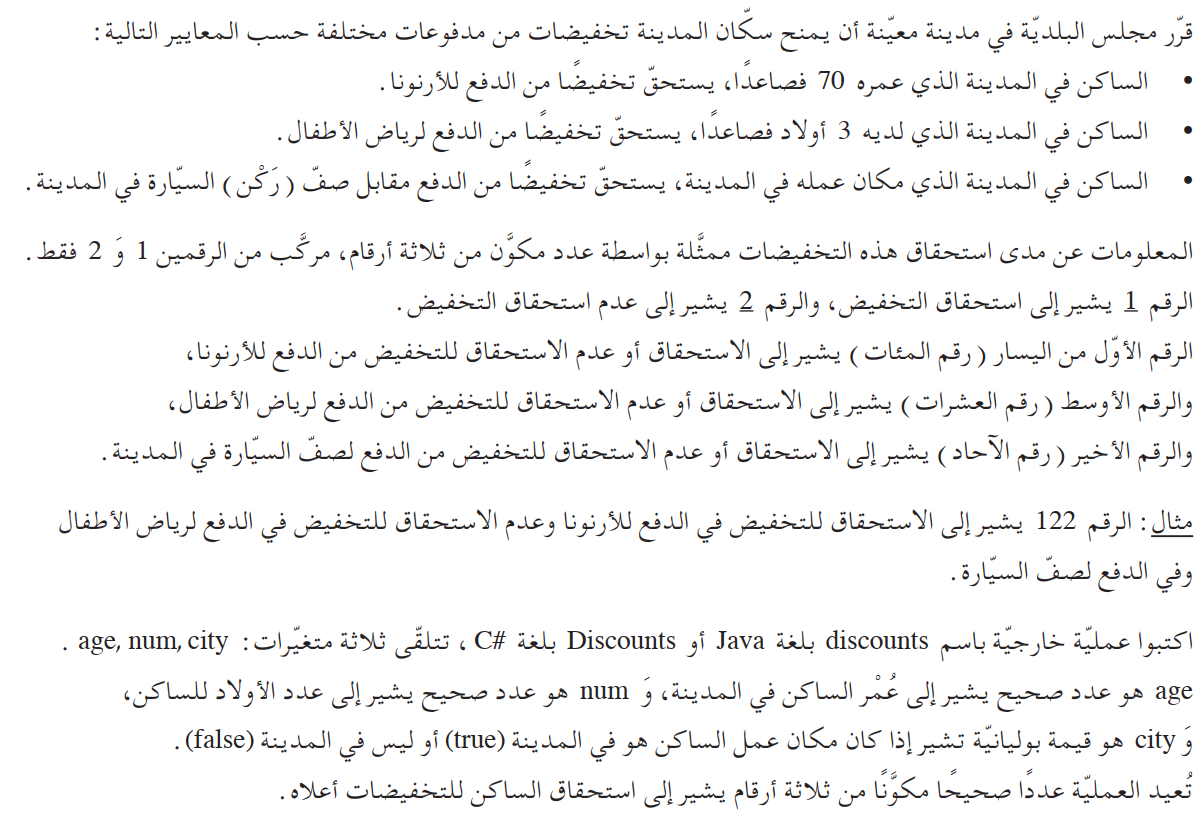
\includegraphics[width=1.1\textwidth]{../../../images/basics_functions_bagrut_question.png}
\end{center}


% قرّر مجلس البلدية في مدينة معيّنة أن يمنح سكان المدينة تخفيضات من مدفوعات مختلفة حسب المعايير التالية:
% \begin{itemize}
%     \item الساكن في المدينة الذي عمره 70 فأصعد، يستحق تخفيضًا من الدفع للأرونا.
%     \item الساكن في المدينة الذي لديه 4 أولاد فأصعد، يستحق تخفيضًا من الدفع لرياض الأطفال.
%     \item الساكن في المدينة الذي مكان عمله في المدينة، يستحق تخفيضًا من الدفع مقابل صفّ (ركن) السيارة في المدينة.
% \end{itemize}

% المعلومات عن مدى استحقاق هذه التخفيضات مُمثّلة بواسطة عدد مكوَّن من ثلاثة أرقام، مركّب من الرقمين 1 و 2 فقط.
% الرقم 1 يشير إلى استحقاق التخفيض، والرقم 2 يشير إلى عدم استحقاق التخفيض.

% \begin{itemize}
%     \item الرقم الأوّل من اليسار (رقم المئات) يشير إلى الاستحقاق أو عدم الاستحقاق للتخفيض من الدفع للأرونا.
%     \item الرقم الأوسط (رقم العشرات) يشير إلى الاستحقاق أو عدم الاستحقاق للتخفيض من الدفع لرياض الأطفال.
%     \item الرقم الأخير (رقم الآحاد) يشير إلى الاستحقاق أو عدم الاستحقاق للتخفيض من الدفع لصفّ السيارة في المدينة.
% \end{itemize}

% مثال: الرقم $122$ يشير إلى الاستحقاق للتخفيض في الدفع للأرونا، وعدم الاستحقاق للتخفيض في الدفع لرياض الأطفال وفي الدفع لصفّ السيارة.

% اكتبوا عملية خارجية باسم \textenglish{Discounts} بلغة \textenglish{C\#} تتلقّى ثلاثة متغيّرات:
% \begin{itemize}
%     \item \textenglish{age} وهو عدد صحيح يشير إلى عمر الساكن في المدينة،
%     \item \textenglish{num} وهو عدد صحيح يشير إلى عدد الأولاد للساكن،
%     \item \textenglish{city} وهو قيمة بوليانية \textenglish{(true/false)} تشير إلى ما إذا كان مكان عمل الساكن هو في المدينة أم لا.
% \end{itemize}

% تُعيد العملية عددًا صحيحًا مكوَّنًا من ثلاثة أرقام يعبّر عن استحقاق الساكن للتخفيضات أعلاه.
% \ifdetailed
% \begin{boxExample}
% \begin{english}
% \begin{minted}{text}
% Input:
% age = 75, num = 2, city = false -> 122
% age = 30, num = 5, city = true  -> 211
% \end{minted}
% \end{english}
% \end{boxExample}
% \fi


\ifwithsols
\begin{boxSolution}
\begin{english}
\begin{minted}{csharp}
public static int Discounts(int age, int num, bool city)
{
    int hundreds = 2;
    int tens = 2;
    int ones = 2;

    if(age >= 70)
    {
        hundreds = 1;
    }
    if(num >= 4)
    {
        tens = 1;
    }
    if (city)
    {
        ones = 1;
    }
    return hundreds * 100 + tens * 10 + ones;
}
public static void Main()
{
    int age = int.Parse(Console.ReadLine());
    int num = int.Parse(Console.ReadLine());
    bool city = bool.Parse(Console.ReadLine());
    Console.WriteLine(Discounts(age, num, city));
}
\end{minted}
\end{english}
\end{boxSolution}
\fi



\end{enumerate}%

\vspace{1cm}
\begin{flushleft}
أرجو لكم وقتًا ممتعًا.

الأستاذ محمود اغبارية.
\end{flushleft}

\end{document}



